\pattern{Flyweight}
\begin{summary}
An object that minimizes memory usage by sharing as much data as possible with
other similar objects.

A way to use objects in large numbers when a simple repeated representation
would use an unacceptable amount of memory. While often some parts of the
object state can be shared. The {\bf Flyweight} pattern describes how to share
objects to allow their use at fine granularity without prohibitive cost. 

Flyweights should be used when a component requires a large number of objects,
the storage costs are high for the number of objects needed, it would be
difficult to maintain the number of objects, and the application does not
depend on object identity.
\end{summary}

\subsubsection{Implementation}
Each ``flyweight'' object is divided into two pieces: the state-dependent
(extrinsic) part, and the state-independent (intrinsic) part. Intrinsic state
is stored (shared) in the Flyweight object. Extrinsic state is stored or
computed by client objects, and passed to the Flyweight when its operations are
invoked. Flyweights are stored in a Factory's repository. The client restrains
herself from creating Flyweights directly, and requests them from the Factory.
Each Flyweight cannot stand on its own. Any attributes that would make sharing
impossible must be supplied by the client whenever a request is made of the
Flyweight.

\comparison{\begin{itemize}
    \item Save memory by reduce the repeat data
    \item Reduction of number of objects to handle when application requires a large number of objects
    \item If the objects are naturally immutable, then impact on performance of using a Flyweight is negligible
    \item Working with Flyweights is easy in a language like Java where all object variables are references and a garbage collector is responsible for removing old objects.
    \end{itemize}
}{\begin{itemize}
    \item Move state outside the object breaks encapsulation
    \item If the object is not naturally immutable, then might affect performance in some case
    \item Little trickier in language like C++ where objects can be allocated as local variables on the stack and destroyed as a result of programmer action.
    \end{itemize}
} %END comparisson

\begin{nfps}
\item[Data integrity] might lose if the data is not intending to share (lost encapsulation)
\item[Performance] might increase in some case like browsing the website with same image, save download same image time. However, in some case the performance might decrease due to save memory that require search the data.
\item[Reusability] since flyweight save common use the same data in just one copy, in that case save certain memory. It is similar to the helper function, that the same data can be used in different class.
\end{nfps}

\begin{center}
    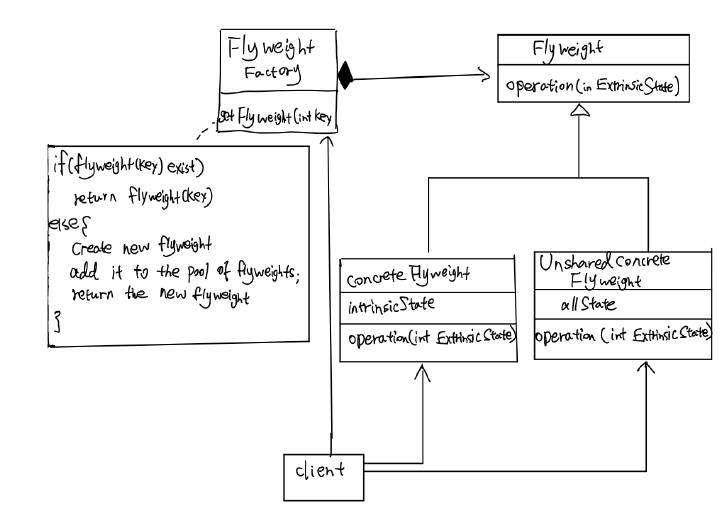
\includegraphics[width=0.4\textwidth]{./flyweight}
\end{center}
